% Options for packages loaded elsewhere
\PassOptionsToPackage{unicode}{hyperref}
\PassOptionsToPackage{hyphens}{url}
\PassOptionsToPackage{dvipsnames,svgnames,x11names}{xcolor}
%
\documentclass[
  authoryear,
  preprint,
  3p]{elsarticle}

\usepackage{amsmath,amssymb}
\usepackage{iftex}
\ifPDFTeX
  \usepackage[T1]{fontenc}
  \usepackage[utf8]{inputenc}
  \usepackage{textcomp} % provide euro and other symbols
\else % if luatex or xetex
  \usepackage{unicode-math}
  \defaultfontfeatures{Scale=MatchLowercase}
  \defaultfontfeatures[\rmfamily]{Ligatures=TeX,Scale=1}
\fi
\usepackage{lmodern}
\ifPDFTeX\else  
    % xetex/luatex font selection
\fi
% Use upquote if available, for straight quotes in verbatim environments
\IfFileExists{upquote.sty}{\usepackage{upquote}}{}
\IfFileExists{microtype.sty}{% use microtype if available
  \usepackage[]{microtype}
  \UseMicrotypeSet[protrusion]{basicmath} % disable protrusion for tt fonts
}{}
\makeatletter
\@ifundefined{KOMAClassName}{% if non-KOMA class
  \IfFileExists{parskip.sty}{%
    \usepackage{parskip}
  }{% else
    \setlength{\parindent}{0pt}
    \setlength{\parskip}{6pt plus 2pt minus 1pt}}
}{% if KOMA class
  \KOMAoptions{parskip=half}}
\makeatother
\usepackage{xcolor}
\setlength{\emergencystretch}{3em} % prevent overfull lines
\setcounter{secnumdepth}{5}
% Make \paragraph and \subparagraph free-standing
\ifx\paragraph\undefined\else
  \let\oldparagraph\paragraph
  \renewcommand{\paragraph}[1]{\oldparagraph{#1}\mbox{}}
\fi
\ifx\subparagraph\undefined\else
  \let\oldsubparagraph\subparagraph
  \renewcommand{\subparagraph}[1]{\oldsubparagraph{#1}\mbox{}}
\fi


\providecommand{\tightlist}{%
  \setlength{\itemsep}{0pt}\setlength{\parskip}{0pt}}\usepackage{longtable,booktabs,array}
\usepackage{calc} % for calculating minipage widths
% Correct order of tables after \paragraph or \subparagraph
\usepackage{etoolbox}
\makeatletter
\patchcmd\longtable{\par}{\if@noskipsec\mbox{}\fi\par}{}{}
\makeatother
% Allow footnotes in longtable head/foot
\IfFileExists{footnotehyper.sty}{\usepackage{footnotehyper}}{\usepackage{footnote}}
\makesavenoteenv{longtable}
\usepackage{graphicx}
\makeatletter
\def\maxwidth{\ifdim\Gin@nat@width>\linewidth\linewidth\else\Gin@nat@width\fi}
\def\maxheight{\ifdim\Gin@nat@height>\textheight\textheight\else\Gin@nat@height\fi}
\makeatother
% Scale images if necessary, so that they will not overflow the page
% margins by default, and it is still possible to overwrite the defaults
% using explicit options in \includegraphics[width, height, ...]{}
\setkeys{Gin}{width=\maxwidth,height=\maxheight,keepaspectratio}
% Set default figure placement to htbp
\makeatletter
\def\fps@figure{htbp}
\makeatother

\makeatletter
\@ifpackageloaded{caption}{}{\usepackage{caption}}
\AtBeginDocument{%
\ifdefined\contentsname
  \renewcommand*\contentsname{Table of contents}
\else
  \newcommand\contentsname{Table of contents}
\fi
\ifdefined\listfigurename
  \renewcommand*\listfigurename{List of Figures}
\else
  \newcommand\listfigurename{List of Figures}
\fi
\ifdefined\listtablename
  \renewcommand*\listtablename{List of Tables}
\else
  \newcommand\listtablename{List of Tables}
\fi
\ifdefined\figurename
  \renewcommand*\figurename{Figure}
\else
  \newcommand\figurename{Figure}
\fi
\ifdefined\tablename
  \renewcommand*\tablename{Table}
\else
  \newcommand\tablename{Table}
\fi
}
\@ifpackageloaded{float}{}{\usepackage{float}}
\floatstyle{ruled}
\@ifundefined{c@chapter}{\newfloat{codelisting}{h}{lop}}{\newfloat{codelisting}{h}{lop}[chapter]}
\floatname{codelisting}{Listing}
\newcommand*\listoflistings{\listof{codelisting}{List of Listings}}
\makeatother
\makeatletter
\makeatother
\makeatletter
\@ifpackageloaded{caption}{}{\usepackage{caption}}
\@ifpackageloaded{subcaption}{}{\usepackage{subcaption}}
\makeatother
\journal{Palaeo3}
\ifLuaTeX
  \usepackage{selnolig}  % disable illegal ligatures
\fi
\usepackage[]{natbib}
\bibliographystyle{elsarticle-harv}
\usepackage{bookmark}

\IfFileExists{xurl.sty}{\usepackage{xurl}}{} % add URL line breaks if available
\urlstyle{same} % disable monospaced font for URLs
\hypersetup{
  pdftitle={Interspecies comparisons of Mg/Ca ratios in limpet shells},
  pdfauthor={Niklas Hausmann; Donna Surge; Francisco Zangrando; Angelica Tivoli; Ivan Briz-Godino},
  pdfkeywords={keyword1, keyword2},
  colorlinks=true,
  linkcolor={blue},
  filecolor={Maroon},
  citecolor={Blue},
  urlcolor={Blue},
  pdfcreator={LaTeX via pandoc}}

\setlength{\parindent}{6pt}
\begin{document}

\begin{frontmatter}
\title{Interspecies comparisons of Mg/Ca ratios in limpet shells}
\author[1]{Niklas Hausmann%
\corref{cor1}%
}
 \ead{niklas@palaeo.eu} 
\author[2]{Donna Surge%
%
}

\author[3]{Francisco Zangrando%
%
}

\author[3]{Angelica Tivoli%
%
}

\author[4]{Ivan Briz-Godino%
%
}


\affiliation[1]{organization={Leibniz Zentrum für
Archäologie},addressline={Ludwig-Lindenschmit-Forum
1},city={Mainz},country={Germany},countrysep={,},postcode={55116},postcodesep={}}
\affiliation[2]{organization={University of North
Carolina},addressline={104 South Road, 225 Geology
Building},city={Chapel Hill,
NC},country={US},countrysep={,},postcode={27599-3315},postcodesep={}}
\affiliation[3]{organization={CONICET (Consejo Nacional de
Investigaciones Científicas y Técnicas)},addressline={Avenida Maipú
305},city={Ushuaia},country={Argentina},countrysep={,},postcode={V9410BJA},postcodesep={}}
\affiliation[4]{organization={},country={Spain},countrysep={,},postcodesep={}}

\cortext[cor1]{Corresponding author}





        
\begin{abstract}
This document is a template demonstrating the Aps format.
\end{abstract}





\begin{keyword}
    keyword1 \sep 
    keyword2
\end{keyword}
\end{frontmatter}
    
\begin{figure}[H]

{\centering 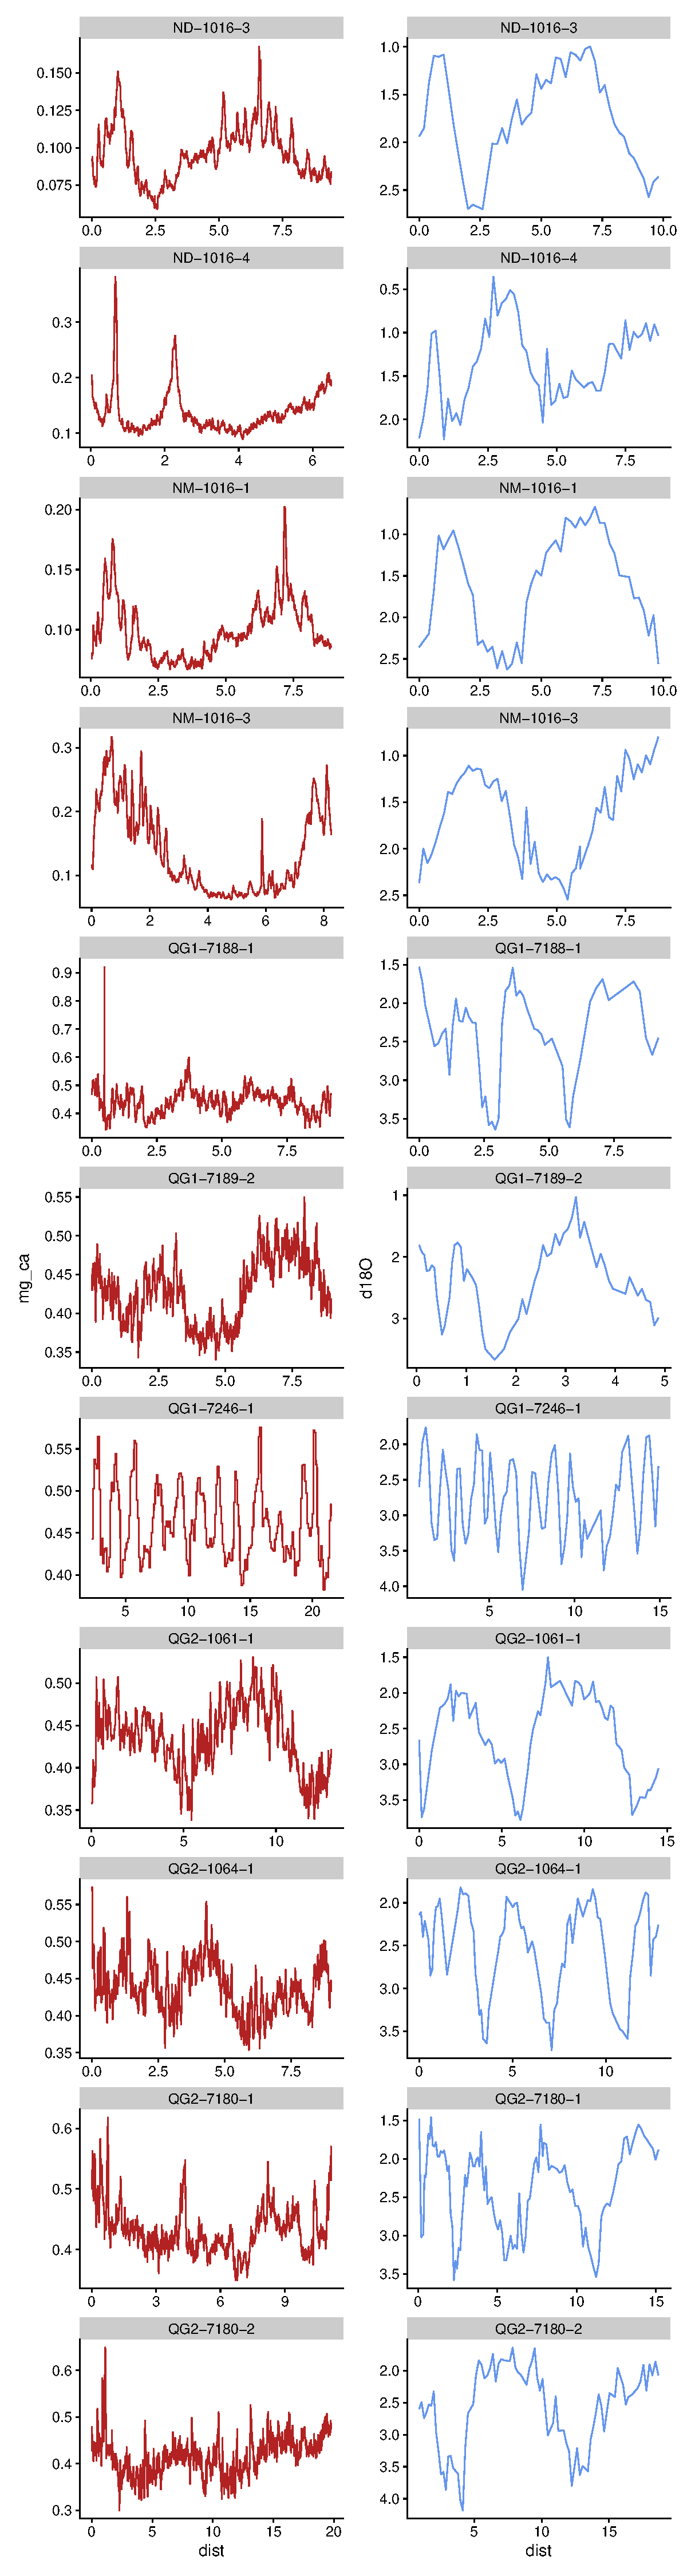
\includegraphics{Manuscript_files/figure-pdf/Raw Data-1.pdf}

}

\caption{Raw Mg/Ca and δ\textsuperscript{18}O Data}

\end{figure}%

\begin{figure}[H]

{\centering 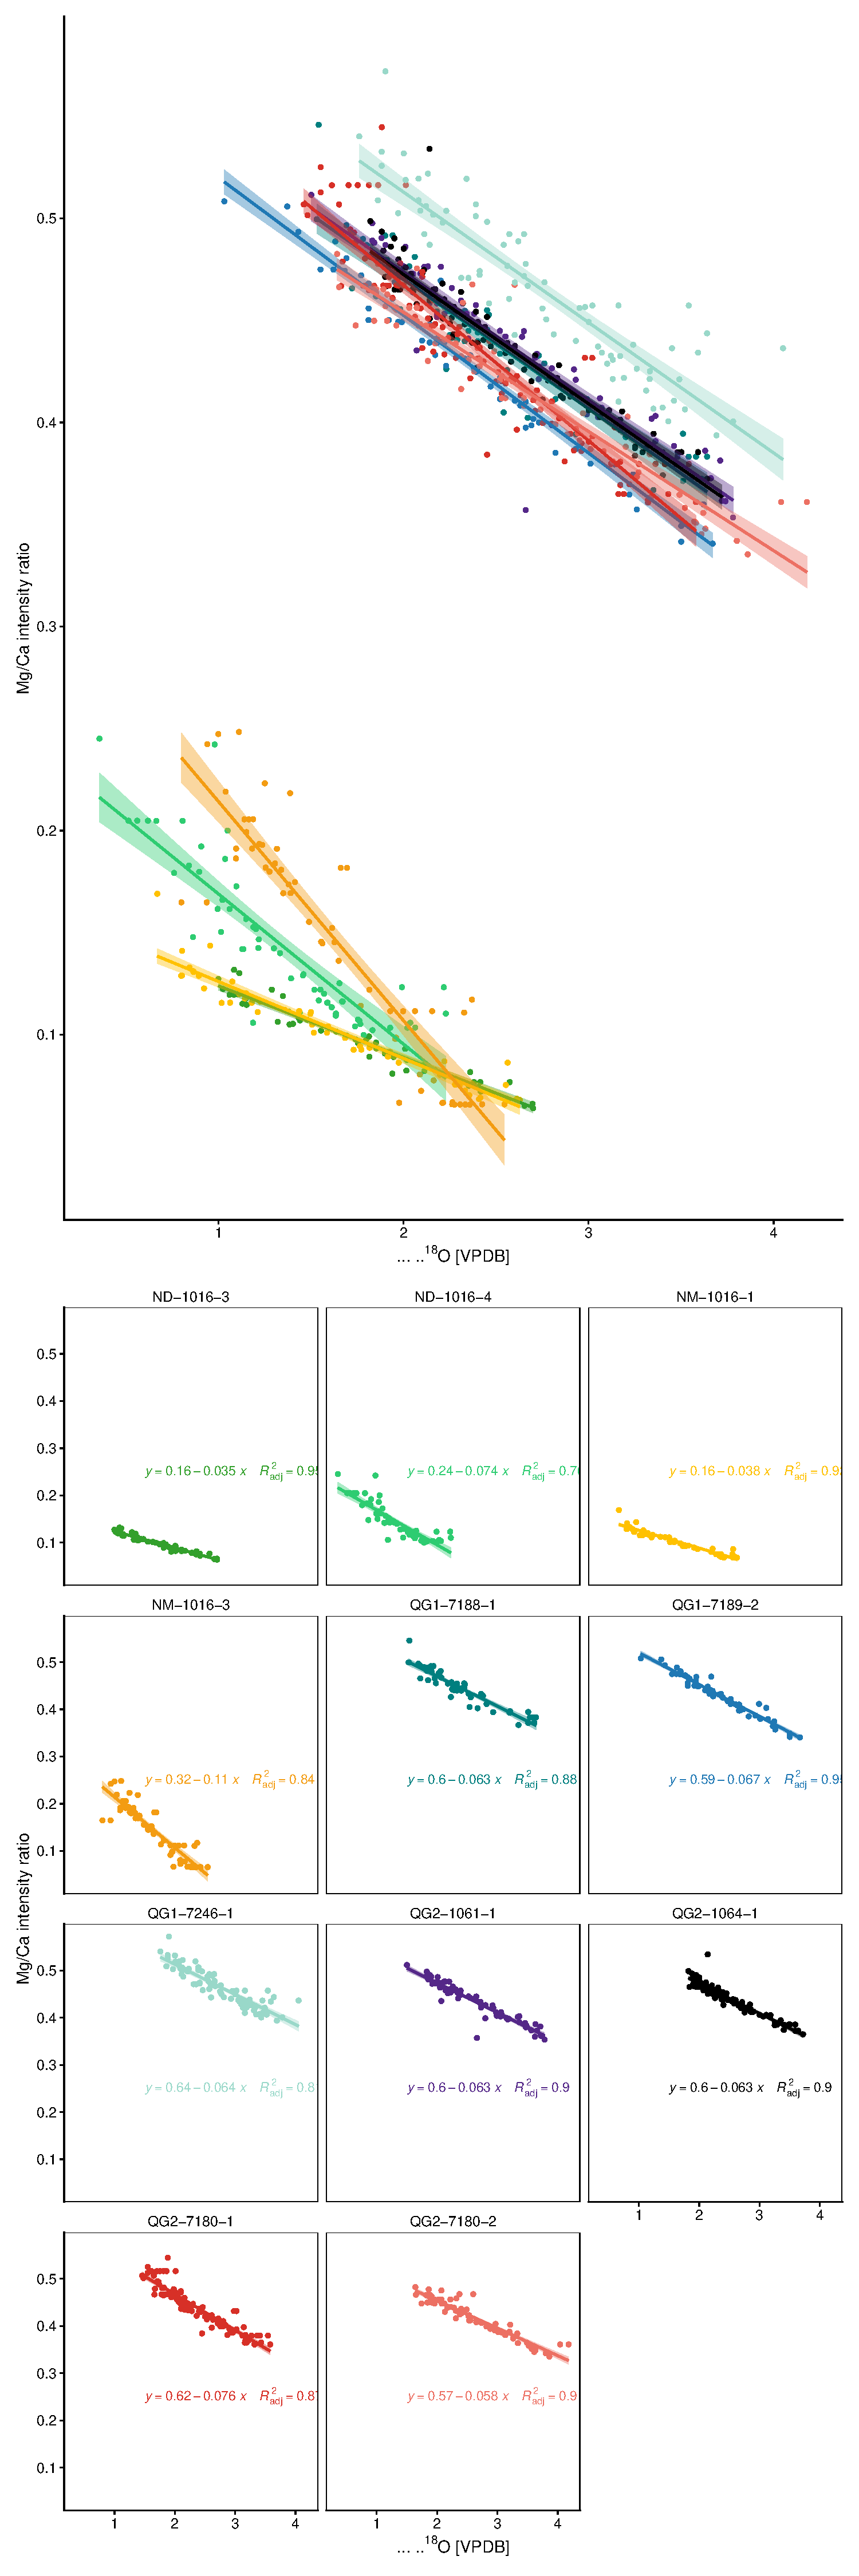
\includegraphics{Manuscript_files/figure-pdf/Correlation Graphs-1.pdf}

}

\caption{Correlation graphs for all specimens}

\end{figure}%


  \bibliography{bibliography.bib}


\end{document}
